\documentclass[11pt, oneside]{article} 
\usepackage{geometry}
\geometry{letterpaper} 
\usepackage{graphicx}
	
\usepackage{amssymb}
\usepackage{amsmath}
\usepackage{parskip}
\usepackage{color}
\usepackage{hyperref}

\graphicspath{{/Users/telliott_admin/Dropbox/Tex/png/}}
% \begin{center} 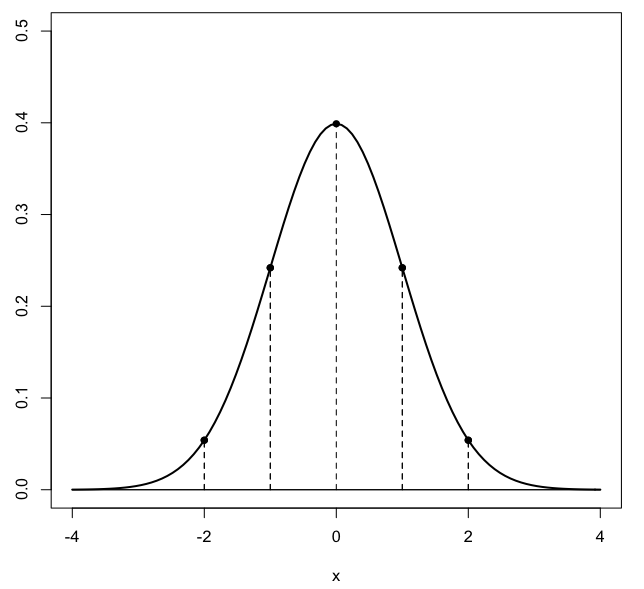
\includegraphics [scale=0.4] {gauss3.png} \end{center}

\title{Irreducible polynomials}
\date{}

\begin{document}
\maketitle
\Large

We will usually represent polynomials as binary numbers.  The irreducible polynomials of degree 3 are
\[ x^3 + x + 1 \]
\[ x^3 + x^2 + 1 \]

For all degrees up to 4, they are

\begin{verbatim}
11    10
111
1011  1101
10011 11001 11101 11111
\end{verbatim}

and $100011011$ for degree 8.  The question is:  how to prove that?

\subsection*{Irreducibility}

How to prove that
\[ x^8 + x^4 + x^3 + x + 1 = 100011011 \]
 is irreducible?

The contrary is that two polynomials multiplied together give this as the result  If that were so, then one at least must be of degree 4 or less since $x^4 * x^4 = x^8$.  

We could generate all the polynomials of degree 4 or less and check them by polynomial division.  That's $2^5 + 2^4 + 2^3 + 2^2 + 2 = 63$ multiplications.  (This is the NCAA basketball tournament problem --- how many games are played?).

There's another way.  If the number above *is* reducible, then its factors must themselves be irreducible polynomials.  

All 9 of them are written above.  We've seen all of them except those of degree 4 before.  Let's show find those, and then test the "irreducible polynomial".

As a warmup, determine all the irreducible polynomials of degree 3 or less:

\subsection*{degree 1}

\begin{verbatim}
10 = x
11 = x + 1
\end{verbatim}

\subsection*{degree 2}

Pairwise multiplication of degree 1 gives degree 2

\begin{verbatim}
100 = x^2
110 = x * (x + 1) = x^2 + x
101 = (x + 1) * (x + 1) = x^2 + 1
\end{verbatim}

These 3 are reducible.  What's left?  There must be 4 total.

\begin{verbatim}
111 = x^2 + x + 1
\end{verbatim}
must be irreducible.

Check by trial division:

\begin{verbatim}
111
10
--
 11
 10
 -- 
  1 r
  
111
11
--
  1 r
\end{verbatim}

I put the $r$ there at the end to show that there was a remainder.

\subsection*{degree 3}

Multiply all degree 2's by all degree 1's.

\begin{verbatim}
1000 = x^3
1100 = x^3 + x^2
1010 = x^3 + x
1110 = x^3 + x^2 + x

1100 = (x + 1) * x^2 = x^3 + x^2
1010 = (x + 1) * (x^2 + x) = x^3 + x
1111 = (x + 1) * (x^2 + 1) = x^3 + x^2 + x + 1
1001 = (x + 1) * (x^2 + x + 1) = x^3 + 1
\end{verbatim}

There are 6 unique ones.  It's easier to see if we write them as binary numbers.

\begin{verbatim}
1000 1100 1010 1110 1111 1001
\end{verbatim}

Rearrange:

\begin{verbatim}
1000 1001 1010
1100 1110 1111
\end{verbatim}

What's missing?  $1011$ and $1101$.

Therefore the two irreducibles at degree 3 are:

\begin{verbatim}
1011 = x^3 + x + 1
1101 = x^3 + x^2 + 1
\end{verbatim}

Check by trial division.  

We could test against all 4 degree 2's.  Because it is degree 3, one degree 2 must be a factor (along with a degree 1).  Alternatively, at least one degree 1 must be a factor.

First: $x^3 + x + 1 = 1011$

\begin{verbatim}
#1
1011
100
 ---
 011 r
 
#2
1011
101
 ---
 001 r
 
#3
1011
110
 ---
 111 
 110
 ---
   1 r
 
#4
1011
111
 ---
 101
 111
 ---
  10 r
\end{verbatim}

Next:  $x^3 + x^2 + 1 = 1101$

\begin{verbatim}
#1
1101
100
 ---
 101
 100
 ---
   1 r
 
#2
1101
101
 ---
 111 
 101
 ---
  10 r
 
#3
1101
110
 ---
   1 r
 
#4
1101
111
 ---
  11 r
\end{verbatim}

We've confirmed the two postulated irreducibles at degree 3.

\subsection*{degree 4}

Self-multiply all four degree 2.

\begin{verbatim}
            100    101    110    111
100 x ->  10000         
101 x     10100  10001      
110 x     11000  11110  10100 
111 x     11100  11011  10010  10101
\end{verbatim}

One duplicate ($10100$).

Also multiply all eight degree 3 by all degree 1:

\begin{verbatim}
              10     11
1000 x ->  10000  11000        
1001 x     10010  11011   
1010 x     10100  10001 
1011 x     10110  11011
1100 x ->  11000  10100      
1101 x     11010  10111   
1110 x     11100  10010
1111 x     11110  10001
\end{verbatim}

Figure out what's missing...

\begin{verbatim}
10000 10001 10010 10011 10100 10101 10110 10111
x     x     x           x     x     o     o     

11000 11001 11010 11011 11100 11101 11110 11111
x           o     x     x           x
\end{verbatim}

So I seem to have four:

\begin{verbatim}
10011 11001 11101 11111
\end{verbatim}

\subsection*{Trial division}

Take all irreducible polynomials of any degree and try to divide the "irreducible" polynomial

Start with the degree 4 irreducibles, and use the trick approach to division:

\begin{verbatim}
#1
100011011
10011
-----
   101011
   10011
   -----
     1101 r

#2
100011011
11001
-----
 10001011
 11001
 -----
  1000011
  11001
  -----
   100111
   11001
   -----
    10101
    11001
    -----
     1100 r

#3
100011011
11101
-----
 11001011
 11101
   -----
   100011
   11101
   -----
    11001
    11101
    -----
      100 r

#4
100011011
11111
-----
 11101011
 11111
   -----
    10011 
    11111
    -----
     1100 r
\end{verbatim}

Degree 3 and smaller are five:

\begin{verbatim}
1101
1011
111
10
11
\end{verbatim}

Try them all

\begin{verbatim}
#1
100011011
1101
----
 10111011
 1101
 ----
  1101011
  1101
  ----
      011 r
      
#2
100011011
1011
----
  1111011
  1011
  ----
   100011
   1011
   ----
     1111
     1011
    -----
      100 r

#3
100011011
111
----
 11011011
 111
 ---
   111011
   111
   ---
      011 r

#4
100011011
10
----
    11011
    10
    ----
     1011
     10
     ----
       11
       10
       --
        1 r

#5
100011011
11
--
 10011011
 11
 --
  1011011
  11
  --
   111011
   11
   --
     1011
     11
     --
      111
      11
      --
        1 r
\end{verbatim}

Checking the last one again, we're asking if ``x + 1`` divides 

\begin{verbatim}
x^8 + x^4 + x^3 + x + 1
(x+1) * x^7 = x^8 + x^7 XOR above -> x^7 + x^4 + x^3 + x + 1
(x+1) * x^6 = x^7 + x^6 XOR above -> x^6 + x^4 + x^3 + x + 1
(x+1) * x^5 = x^6 + x^5 XOR above -> x^5 + x^4 + x^3 + x + 1
(x+1) * x^4 = x^5 + x^4 XOR above -> x^3 + x + 1
(x+1) * x^2 = x^3 + x^2 XOR above ->x^2 + x + 1
(x+1) * x = x^2 + x XOR above -> 1
\end{verbatim}

So, no, it doesn't.

There's got to be a better way.  We can do the graphical method:

\begin{verbatim}
100011011
11
--
 10011011
 11
 --
  1011011
  11
  --
   111011
   11
   --
     1011
     11
     -- 
      111
      11
      --
        1 r
\end{verbatim}

A better way is to code it.  I wrote a script with a function which does "string" division.  

Given the irreducible polynomial as $'100011011'$` and any of the irreducibles up to degree 4 as

\begin{verbatim}
L = ['10','11',
     '111',
     '1011','1101',
     '10011', '11001', '11101', '11111']

\end{verbatim}

it prints something like

\begin{verbatim}
string division
 100011011
 11001
  10001011
  11001
   1000011
   11001
    100111
    11001
     10101
     11001
      1100
result:  1100
\end{verbatim}

Comparing the output with the calculations I did by hand above, I found four errors, and one bug!

I also found 30 irreducible polynomials of degree 8.  Here are the first four:

\begin{verbatim}
100011011
100011101
100101011
100101101
..
\end{verbatim}

You will recognize our old friend as the first one, with the smallest binary representation.

\end{document}